\section{Qualitative regressors}


\begin{frame}{Qualitative regressors}
    \begin{itemize}
        \item So far every regressor has been quantitative: speed, temperature, delivery volume.
        \item Many important predictors are qualitative (categorical): sex, region, treatment group, machine type.
        \item A category has no numerical value, so it cannot enter $\bX$ as it is.
        \item \textbf{Question:} how can we put ``tool type A or B'' into a regression model?
        % Answer: encode it with a numeric variable that takes the values 0 and 1 (indicator / dummy variable).
    \end{itemize}
\end{frame}


\begin{frame}{Example dataset: tool life data}
    \begin{itemize}
        \item $y$: hours of tool life; $x_1$: lathe speed (rpm); two tool types, A and B, $n = 20$.
    \end{itemize}

    \vspace{0.5em}

    \begin{center}
        \mode<presentation>{\footnotesize}
        \begin{tabular}{rrr@{\hspace{3em}}rrr}
            \toprule
            \multicolumn{3}{c}{Tool type A} & \multicolumn{3}{c}{Tool type B} \\
            \cmidrule(lr){1-3} \cmidrule(lr){4-6}
            $i$ & $y$ & $x_1$ & $i$ & $y$ & $x_1$ \\
            \midrule
            1  & 18.73 & 610  & 11 & 30.16 & 670  \\
            2  & 14.52 & 950  & 12 & 27.09 & 770  \\
            3  & 17.43 & 720  & 13 & 25.40 & 880  \\
            4  & 14.54 & 840  & 14 & 26.05 & 1000 \\
            5  & 13.44 & 980  & 15 & 33.49 & 760  \\
            6  & 24.39 & 530  & 16 & 35.62 & 590  \\
            7  & 13.34 & 680  & 17 & 26.07 & 910  \\
            8  & 22.71 & 540  & 18 & 36.78 & 650  \\
            9  & 12.68 & 890  & 19 & 34.95 & 810  \\
            10 & 19.32 & 730  & 20 & 43.67 & 500  \\
            \bottomrule
        \end{tabular}
    \end{center}
\end{frame}


\begin{frame}{What happens if we ignore tool type?}
    \begin{columns}[T]
        \begin{column}{0.54\textwidth}
            \centering
            \mode<presentation>{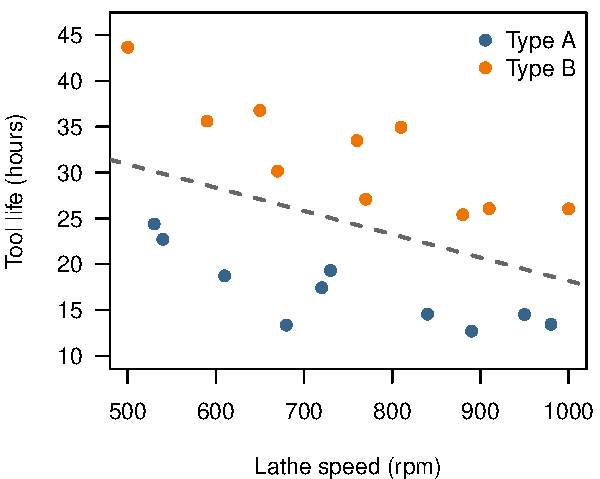
\includegraphics[width=\linewidth]{figures/tool-slr.pdf}}
            \mode<article>{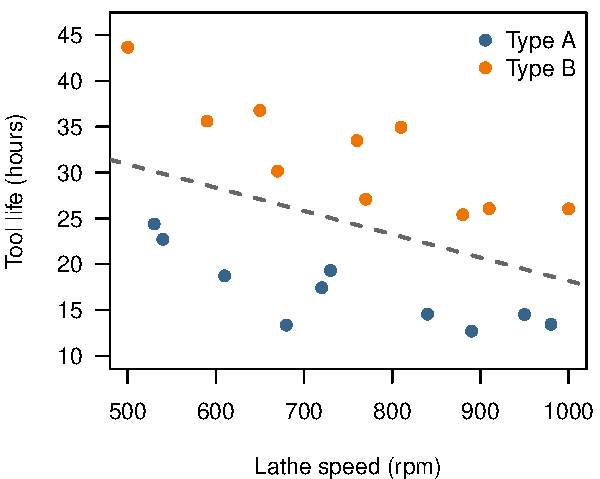
\includegraphics[width=0.6\linewidth]{figures/tool-slr.pdf}}
        \end{column}
        \begin{column}{0.46\textwidth}
            \begin{itemize}
                \item Simple linear regression of $y$ on $x_1$ (dashed): $\hat{y} = 43.62 - 0.0254\, x_1$.
                \item $R^2 = 0.186$, $\hat{\sigma} = 8.44$.
                \item The points split into two clusters: type B tools last longer at every speed.
                \item Tool type is a missing regressor; the residuals carry its effect.
            \end{itemize}
        \end{column}
    \end{columns}
\end{frame}


\section{Indicator variables}


\begin{frame}{Indicator (dummy) variable}
    \begin{itemize}
        \item An indicator variable encodes membership in a category with the values $0$ and $1$.
        \item For tool type:
    \end{itemize}
    \[
        x_2 =
        \begin{cases}
            0 & \text{if the observation is from tool type A},\\
            1 & \text{if the observation is from tool type B}.
        \end{cases}
    \]
    \begin{itemize}
        \item Type A is coded $0$: it is the \textbf{reference} (baseline) category.
    \end{itemize}
\end{frame}



\begin{frame}{Tool life data with the indicator column}
    \centering
    \mode<presentation>{\footnotesize}
    \begin{tabular}{rrrr@{\hspace{2.5em}}rrrr}
        \toprule
        \multicolumn{4}{c}{Tool type A} & \multicolumn{4}{c}{Tool type B} \\
        \cmidrule(lr){1-4} \cmidrule(lr){5-8}
        $i$ & $y$ & $x_1$ & $x_2$ & $i$ & $y$ & $x_1$ & $x_2$ \\
        \midrule
        1  & 18.73 & 610  & 0 & 11 & 30.16 & 670  & 1 \\
        2  & 14.52 & 950  & 0 & 12 & 27.09 & 770  & 1 \\
        3  & 17.43 & 720  & 0 & 13 & 25.40 & 880  & 1 \\
        4  & 14.54 & 840  & 0 & 14 & 26.05 & 1000 & 1 \\
        5  & 13.44 & 980  & 0 & 15 & 33.49 & 760  & 1 \\
        6  & 24.39 & 530  & 0 & 16 & 35.62 & 590  & 1 \\
        7  & 13.34 & 680  & 0 & 17 & 26.07 & 910  & 1 \\
        8  & 22.71 & 540  & 0 & 18 & 36.78 & 650  & 1 \\
        9  & 12.68 & 890  & 0 & 19 & 34.95 & 810  & 1 \\
        10 & 19.32 & 730  & 0 & 20 & 43.67 & 500  & 1 \\
        \bottomrule
    \end{tabular}
 
    \vspace{0.8em}
    \raggedright
    $x_2 = 0$ for tool type A and $x_2 = 1$ for tool type B; $x_2$ is a new column of $\bX$ next to $\mathbf{1}$ and $x_1$.
\end{frame}


\begin{frame}{Model with one quantitative regressor and one indicator}
    \begin{itemize}
        \item Regress $y$ on speed $x_1$ and the indicator $x_2$:
    \end{itemize}
    \[
        y_i = \beta_0 + \beta_1 x_{i1} + \beta_2 x_{i2} + \varepsilon_i, \qquad \varepsilon_i \sim N(0, \sigma^2).
    \]
    \begin{itemize}
        \item This is an ordinary multiple linear regression; $\bX$ has columns $\mathbf{1}$, $\bx_1$, $\bx_2$, and OLS applies unchanged.
        \item Only the interpretation of the coefficient on $x_2$ is new.
    \end{itemize}
\end{frame}


\begin{frame}{Two regression lines from one model}
    \begin{itemize}
        \item Setting $x_2 = 0$ and $x_2 = 1$ gives the mean response for each tool type:
    \end{itemize}
    \begin{align*}
        \text{Type A } (x_2 = 0)\colon \quad \mathbb{E}(y \mid x_1) &= \beta_0 + \beta_1 x_1, \\
        \text{Type B } (x_2 = 1)\colon \quad \mathbb{E}(y \mid x_1) &= (\beta_0 + \beta_2) + \beta_1 x_1.
    \end{align*}
    \begin{itemize}
        \item The lines have the same slope $\beta_1$ and intercepts that differ by $\beta_2$: the lines are \textbf{parallel}.
        \item $\beta_2$ is the difference in mean tool life between type B and type A at any fixed speed.
    \end{itemize}
\end{frame}


\begin{frame}{Geometry: parallel lines}
    \begin{columns}[T]
        \begin{column}{0.5\textwidth}
            \begin{center}
                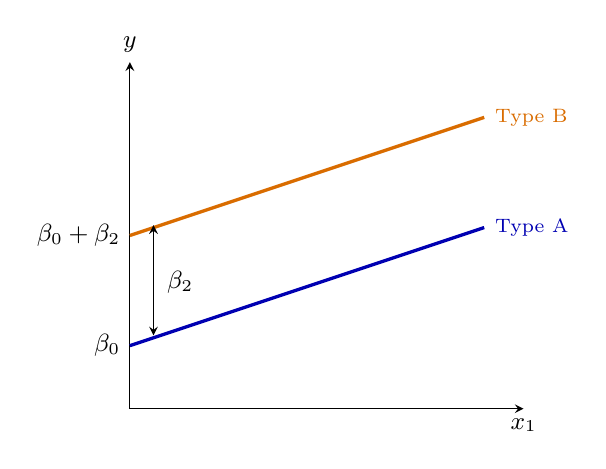
\begin{tikzpicture}[>=stealth]
                    \draw[->] (0,0) -- (5,0) node[below] {\small $x_1$};
                    \draw[->] (0,0) -- (0,4.4) node[above] {\small $y$};
                    \draw[very thick, blue!70!black] (0,0.8) -- (4.5,2.3) node[right] {\scriptsize Type A};
                    \draw[very thick, orange!85!black] (0,2.2) -- (4.5,3.7) node[right] {\scriptsize Type B};
                    \draw[<->] (0.3,0.93) -- (0.3,2.33);
                    \node[anchor=west] at (0.35,1.6) {\small $\beta_2$};
                    \node[anchor=east] at (0,0.8) {\small $\beta_0$};
                    \node[anchor=east] at (0,2.2) {\small $\beta_0 + \beta_2$};
                \end{tikzpicture}
            \end{center}
        \end{column}
        \begin{column}{0.5\textwidth}
            \begin{itemize}
                \item The indicator shifts the intercept only.
                \item The effect of the category does not depend on $x_1$: the vertical gap is $\beta_2$ everywhere.
                \item This is a strong assumption; we will test it with an interaction term.
            \end{itemize}
        \end{column}
    \end{columns}
\end{frame}


\begin{frame}{Tool life: fitted parallel-lines model}
    \[
        \hat{y} = 36.986 - 0.0266\, x_1 + 15.004\, x_2 .
    \]
    \centering
    \small
    \begin{tabular}{lrrr}
        \toprule
        Predictor & Estimate & Std.\ error & $t$ \\
        \midrule
        Intercept & $36.986$ & $3.510$ & $10.54$ \\
        $x_1$ (speed) & $-0.0266$ & $0.0045$ & $-5.89$ \\
        $x_2$ (type B) & $15.004$ & $1.360$ & $11.04$ \\
        \bottomrule
    \end{tabular}

    \vspace{0.8em}
    \raggedright
    $R^2 = 0.900$, \quad $\hat{\sigma} = 3.04$ on $17$ degrees of freedom.
\end{frame}


\begin{frame}{Interpreting the coefficients}
    \begin{itemize}
        \item \textbf{Question:} what do $\hat{\beta}_1 = -0.0266$ and $\hat{\beta}_2 = 15.004$ mean in this problem?
        % Answer: beta1: for either tool type, each extra rpm lowers mean tool life by 0.0266 hours (about 2.66 hours per 100 rpm).
        % Answer: beta2: at any fixed speed, type B tools last 15.0 hours longer on average than type A tools.
    \end{itemize}
\end{frame}


\begin{frame}{Fitted lines and data}
    \begin{columns}[T]
        \begin{column}{0.54\textwidth}
            \centering
            \mode<presentation>{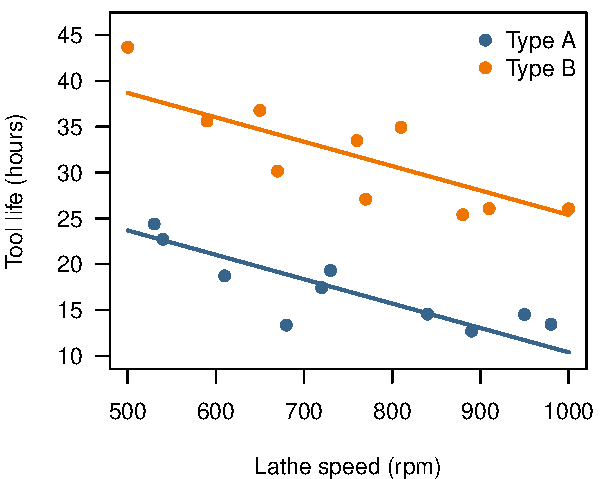
\includegraphics[width=\linewidth]{figures/tool-parallel.pdf}}
            \mode<article>{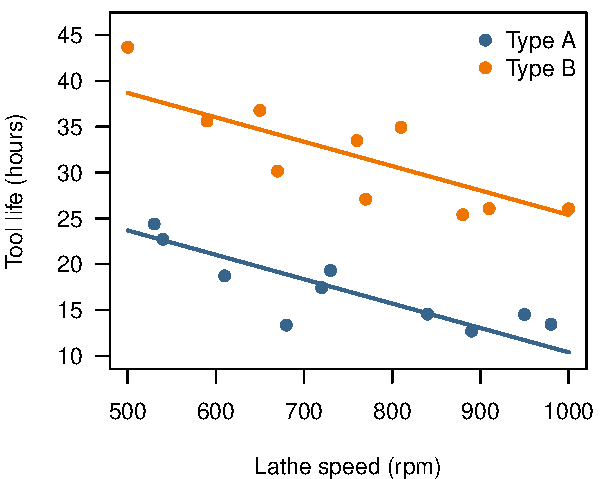
\includegraphics[width=0.6\linewidth]{figures/tool-parallel.pdf}}
        \end{column}
        \begin{column}{0.46\textwidth}
            \begin{itemize}
                \item Type A: $\hat{y} = 36.99 - 0.0266\, x_1$.
                \item Type B: $\hat{y} = 51.99 - 0.0266\, x_1$.
                \item Adding the indicator raises $R^2$ from $0.186$ to $0.900$ and cuts $\hat{\sigma}$ from $8.44$ to $3.04$.
            \end{itemize}
        \end{column}
    \end{columns}
\end{frame}


\section{Inference on the indicator coefficient}


\begin{frame}{Full and reduced models}
    \begin{itemize}
        \item A hypothesis $H_0$ about the coefficients, e.g.\ that some of them are zero, defines a simpler model.
        \item \textbf{Full model (FM):} all terms; $p$ parameters.
        \item \textbf{Reduced model (RM):} the FM with $H_0$ imposed; $p - q$ parameters, where $q$ is the number of restrictions in $H_0$.
        \item The RM is \emph{nested} in the FM: every RM is a special case of the FM.
    \end{itemize}
    \vspace{0.5em}
    Example: $H_0\colon \beta_2 = 0$ ($q = 1$).
    \begin{align*}
        \text{FM}\colon\quad y &= \beta_0 + \beta_1 x_1 + \beta_2 x_2 + \varepsilon, \\
        \text{RM}\colon\quad y &= \beta_0 + \beta_1 x_1 + \varepsilon .
    \end{align*}
\end{frame}


\begin{frame}{Extra sum of squares}
    \begin{itemize}
        \item Least squares searches over all coefficient values allowed by the model; the FM allows more, so
    \end{itemize}
    \[
        \SSRes(\text{RM}) \ge \SSRes(\text{FM}).
    \]
    \begin{itemize}
        \item The difference is the \textbf{extra sum of squares}: the increase in the residual sum of squares caused by imposing $H_0$,
    \end{itemize}
    \[
        \SSRes(\text{RM}) - \SSRes(\text{FM}) \ge 0 .
    \]
    \begin{itemize}
        \item Small increase: the dropped terms add little, and $H_0$ is plausible. Large increase: the dropped terms matter.
        \item \textbf{Question:} how large is ``large''?
        % Answer: compare it to the noise level, i.e.\ to an estimate of sigma^2 from the full model, MSRes(FM) = SSRes(FM)/(n-p); and divide by q to get the increase per restriction.
    \end{itemize}
\end{frame}


\begin{frame}{$F$-test for nested models}
    \begin{itemize}
        \item Under $H_0$, with $n$ observations, $p$ parameters in the FM and $q$ restrictions:
    \end{itemize}
    \[
        F_0 = \frac{\left[\SSRes(\text{RM}) - \SSRes(\text{FM})\right] / q}{\SSRes(\text{FM}) / (n - p)} \sim F_{q,\, n-p}.
    \]
    \begin{itemize}
        \item Numerator: increase in $\SSRes$ per restriction. Denominator: $\mathit{MS}_{\mathrm{Res}}$ of the FM, an estimate of $\sigma^2$.
        \item Reject $H_0$ at level $\alpha$ if $F_0 > F_{\alpha,\, q,\, n-p}$.
        \item For $q = 1$ the test is equivalent to the two-sided $t$-test of the coefficient, with $F_0 = t_0^2$.
    \end{itemize}
\end{frame}


\begin{frame}{Inference on the indicator coefficient}
    \begin{itemize}
        \item $H_0\colon \beta_2 = 0$ (the two tool types have the same mean life at every speed) is tested with the usual $t$-test; here $t_0 = 11.04$ on $17$ df.
        \item Equivalently, use the $F$-test with FM: $y = \beta_0 + \beta_1 x_1 + \beta_2 x_2 + \varepsilon$ and RM: $y = \beta_0 + \beta_1 x_1 + \varepsilon$ (speed only); here $q = 1$, $n - p = 17$:
    \end{itemize}
    \begin{align*}
        F_0 &= \frac{\left[\SSRes(\text{RM}) - \SSRes(\text{FM})\right] / 1}{\SSRes(\text{FM}) / 17}
        = \frac{(1282.08 - 157.05)/1}{157.05/17} = 121.8, \\
        F_0 &= t_0^2 .
    \end{align*}
    \begin{itemize}
        \item Reject $H_0$: tool type is strongly associated with tool life after adjusting for speed.
    \end{itemize}
\end{frame}


\section{Factors with more than two levels}


\begin{frame}{Categorical regressor with $k$ levels}
    \begin{itemize}
        \item A factor with $k$ levels is represented by $k-1$ indicator variables.
        \item The level without an indicator is the reference level.
        \item Suppose there were three tool types A, B, C (hypothetical extension), with A as reference:
    \end{itemize}
    \[
        x_2 =
        \begin{cases}
            1 & \text{if type B},\\
            0 & \text{otherwise},
        \end{cases}
        \qquad
        x_3 =
        \begin{cases}
            1 & \text{if type C},\\
            0 & \text{otherwise}.
        \end{cases}
    \]
\end{frame}


\begin{frame}{Coding and interpretation for $k = 3$}
    \[
        y = \beta_0 + \beta_1 x_1 + \beta_2 x_2 + \beta_3 x_3 + \varepsilon
    \]
    \centering
    \small
    \begin{tabular}{lrrl}
        \toprule
        Type & $x_2$ & $x_3$ & $\mathbb{E}(y \mid x_1)$ \\
        \midrule
        A & 0 & 0 & $\beta_0 + \beta_1 x_1$ \\
        B & 1 & 0 & $(\beta_0 + \beta_2) + \beta_1 x_1$ \\
        C & 0 & 1 & $(\beta_0 + \beta_3) + \beta_1 x_1$ \\
        \bottomrule
    \end{tabular}

    \vspace{0.8em}
    \raggedright
    $\beta_2$ and $\beta_3$ are the differences of B and C from the reference A, at fixed $x_1$. The difference between B and C is $\beta_2 - \beta_3$.
\end{frame}


\begin{frame}{The dummy variable trap}
    \begin{itemize}
        \item Suppose we include all $k = 3$ indicators $\mathbf{d}_A, \mathbf{d}_B, \mathbf{d}_C$ together with an intercept.
        \item Every observation belongs to exactly one type, so
    \end{itemize}
    \begin{align*}
        \mathbf{1} &= \mathbf{d}_A + \mathbf{d}_B + \mathbf{d}_C, \\
        \operatorname{rank}(\bX) &= 4 < 5 \text{ columns}.
    \end{align*}
    \begin{itemize}
        \item $\bX^\top \bX$ is singular: the normal equations have no unique solution and $\bbeta$ is not identifiable.
        \item Remedy: drop one indicator (use $k-1$), or drop the intercept (then each coefficient is a level-specific intercept).
    \end{itemize}
\end{frame}


\begin{frame}{Question: counting indicators}
    \begin{itemize}
        \item A factor has $4$ levels and the model includes an intercept. How many indicators are needed? How many if the intercept is removed, and how does the meaning of the coefficients change?
        % Answer: 3 indicators with the intercept. Without the intercept, 4 indicators; each coefficient is then the mean response for that level (at x = 0 for any quantitative regressors).
    \end{itemize}
\end{frame}


\begin{frame}{Choice of reference level}
    \begin{itemize}
        \item Changing the reference level changes the coefficients, not the model.
        \item With reference C instead of A, the model $\beta_0 + \beta_1 x_1 + \beta_2 x_2 + \beta_3 x_3$ is re-expressed as
    \end{itemize}
    \begin{align*}
        \beta_0' &= \beta_0 + \beta_3, \\
        \beta_{A}' &= -\beta_3, \\
        \beta_{B}' &= \beta_2 - \beta_3 .
    \end{align*}
    \begin{itemize}
        \item Fitted values, residuals, $\SSRes$, $R^2$ and the overall $F$-test of the factor are identical for every choice of reference level.
        \item Choose the reference level that makes the comparisons of interest direct (e.g.\ a control group).
    \end{itemize}
\end{frame}


\begin{frame}{Testing the factor as a whole}
    \begin{itemize}
        \item Individual $t$-tests compare one level with the reference only.
        \item To test whether the factor matters at all, $H_0\colon \beta_2 = \beta_3 = 0$, use the partial $F$-test:
    \end{itemize}
    \[
        F_0 = \frac{\left[\SSRes(\text{RM}) - \SSRes(\text{FM})\right]/(k-1)}{\SSRes(\text{FM})/(n - p)} \sim F_{k-1,\, n-p} \quad \text{under } H_0,
    \]
    \begin{itemize}
        \item where the reduced model omits all $k-1$ indicators and $p$ is the number of parameters of the full model.
    \end{itemize}
\end{frame}


\begin{frame}{Indicator variables versus allocated codes}
    \begin{itemize}
        \item Tempting alternative: one regressor with codes A $= 1$, B $= 2$, C $= 3$ (allocated codes).
        \item This forces $\mathbb{E}(y)$ to change by the same amount $\beta$ from A to B and from B to C, as if the levels were equally spaced on a numeric scale.
        \item For nominal categories that ordering and spacing is arbitrary; recoding to A $= 1$, C $= 2$, B $= 3$ would change the fit.
        \item Indicator variables impose no such structure: each level gets its own mean shift.
        \item Allocated codes are defensible only when the levels are genuinely ordered and roughly equally spaced.
    \end{itemize}
\end{frame}


\section{Interaction terms}


\begin{frame}{Do both tool types respond to speed in the same way?}
    \begin{itemize}
        \item The parallel-lines model assumes that increasing speed shortens life by the same amount for tool types A and B.
        \item \textbf{Question:} how can we let the slope on $x_1$ differ between the two types?
        % Answer: add the product x1*x2 (interaction term); its coefficient is the difference in slopes.
    \end{itemize}
\end{frame}


\begin{frame}{Indicator $\times$ quantitative interaction}
    \begin{itemize}
        \item Add the product of the indicator and the quantitative regressor:
    \end{itemize}
    \[
        y_i = \beta_0 + \beta_1 x_{i1} + \beta_2 x_{i2} + \beta_3 x_{i1} x_{i2} + \varepsilon_i .
    \]
    \begin{itemize}
        \item The effect of $x_1$ now depends on the category, and the effect of the category depends on $x_1$.
    \end{itemize}
\end{frame}


\begin{frame}{Group-specific lines}
    \begin{align*}
        \text{Type A } (x_2 = 0)\colon \quad \mathbb{E}(y \mid x_1) &= \beta_0 + \beta_1 x_1, \\
        \text{Type B } (x_2 = 1)\colon \quad \mathbb{E}(y \mid x_1) &= (\beta_0 + \beta_2) + (\beta_1 + \beta_3)\, x_1 .
    \end{align*}
    \begin{itemize}
        \item $\beta_2$: difference in intercepts; $\beta_3$: difference in slopes.
        \item The difference between the types at speed $x_1$ is $\beta_2 + \beta_3 x_1$; it changes linearly with $x_1$.
    \end{itemize}
\end{frame}


\begin{frame}{Geometry: non-parallel lines}
    \begin{columns}[T]
        \begin{column}{0.5\textwidth}
            \begin{center}
                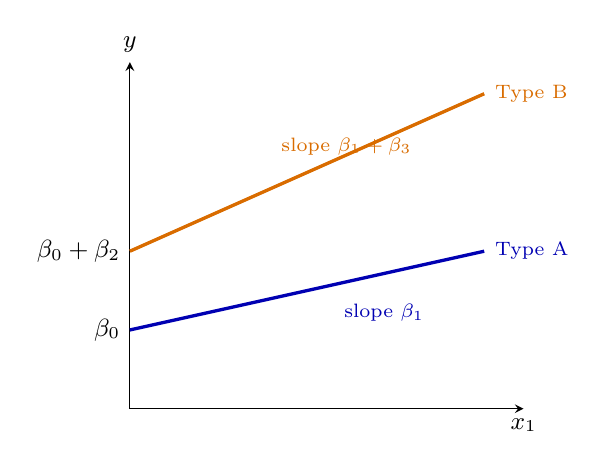
\begin{tikzpicture}[>=stealth]
                    \draw[->] (0,0) -- (5,0) node[below] {\small $x_1$};
                    \draw[->] (0,0) -- (0,4.4) node[above] {\small $y$};
                    \draw[very thick, blue!70!black] (0,1.0) -- (4.5,2.0) node[right] {\scriptsize Type A};
                    \draw[very thick, orange!85!black] (0,2.0) -- (4.5,4.0) node[right] {\scriptsize Type B};
                    \node[anchor=east] at (0,1.0) {\small $\beta_0$};
                    \node[anchor=east] at (0,2.0) {\small $\beta_0 + \beta_2$};
                    \node[blue!70!black, anchor=north west] at (2.6,1.45) {\scriptsize slope $\beta_1$};
                    \node[orange!85!black, anchor=south east] at (3.7,3.1) {\scriptsize slope $\beta_1 + \beta_3$};
                \end{tikzpicture}
            \end{center}
        \end{column}
        \begin{column}{0.5\textwidth}
            \begin{itemize}
                \item Two free intercepts and two free slopes.
                \item The vertical gap between the lines grows with $x_1$ when $\beta_3 > 0$.
                \item The lines cross at $x_1 = -\beta_2 / \beta_3$ (if this lies in the range of the data, the ranking of the types reverses).
            \end{itemize}
        \end{column}
    \end{columns}
\end{frame}


\begin{frame}{Tool life: fitted interaction model}
    \[
        \hat{y} = 32.775 - 0.0210\, x_1 + 23.971\, x_2 - 0.0119\, x_1 x_2 .
    \]
    \centering
    \small
    \begin{tabular}{lrrr}
        \toprule
        Predictor & Estimate & Std.\ error & $t$ \\
        \midrule
        Intercept & $32.775$ & $4.634$ & $7.07$ \\
        $x_1$ (speed) & $-0.0210$ & $0.0061$ & $-3.45$ \\
        $x_2$ (type B) & $23.971$ & $6.769$ & $3.54$ \\
        $x_1 x_2$ & $-0.0119$ & $0.0088$ & $-1.35$ \\
        \bottomrule
    \end{tabular}

    \vspace{0.8em}
    \raggedright
    $R^2 = 0.911$, \quad $\hat{\sigma} = 2.97$ on $16$ degrees of freedom.
\end{frame}


\begin{frame}{Tool life: different slopes by tool type}
    \begin{columns}[T]
        \begin{column}{0.54\textwidth}
            \centering
            \mode<presentation>{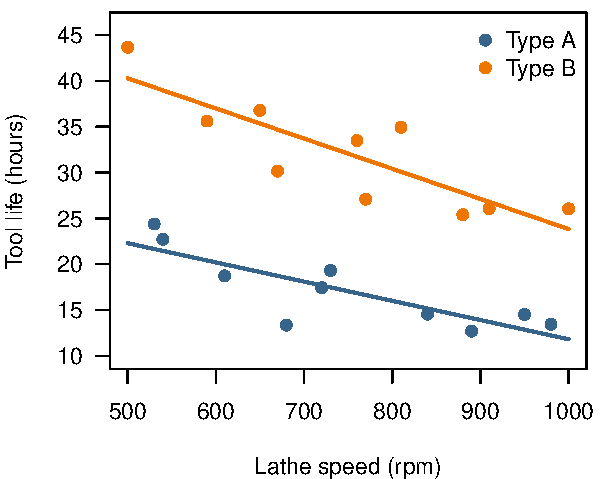
\includegraphics[width=\linewidth]{figures/tool-interaction.pdf}}
            \mode<article>{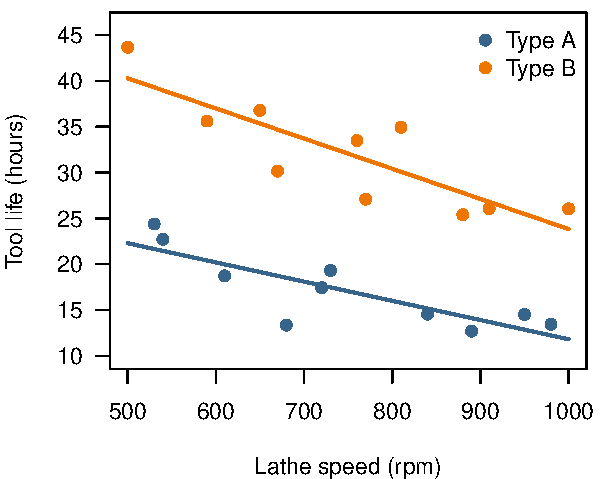
\includegraphics[width=0.6\linewidth]{figures/tool-interaction.pdf}}
        \end{column}
        \begin{column}{0.46\textwidth}
            \begin{itemize}
                \item Type A: $\hat{y} = 32.78 - 0.0210\, x_1$.
                \item Type B: $\hat{y} = 56.75 - 0.0329\, x_1$.
                \item The estimated slope is steeper for type B ($\hat{\beta}_3 = -0.0119$), so the lines converge as speed increases.
                \item Is this difference larger than sampling variation?
            \end{itemize}
        \end{column}
    \end{columns}
\end{frame}


\begin{frame}{Testing the interaction}
    \begin{itemize}
        \item $H_0\colon \beta_3 = 0$ (parallel lines): is the interaction term needed beyond $x_1$ and $x_2$? Compare nested models, with $q = 1$ and $n - p = 16$:
    \end{itemize}
    \begin{align*}
        \text{FM}\colon\quad y &= \beta_0 + \beta_1 x_1 + \beta_2 x_2 + \beta_3 x_1 x_2 + \varepsilon, \\
        \text{RM}\colon\quad y &= \beta_0 + \beta_1 x_1 + \beta_2 x_2 + \varepsilon .
    \end{align*}
\end{frame}


\begin{frame}{Testing the interaction: result}
    \begin{align*}
        F_0 &= \frac{\left[\SSRes(\text{RM}) - \SSRes(\text{FM})\right] / 1}{\SSRes(\text{FM}) / 16}
        = \frac{(157.05 - 140.98)/1}{140.98/16} = 1.82, \\
        t_0 &= -1.35 \quad (t_0^2 = F_0), \qquad p\text{-value} = 0.196 .
    \end{align*}
    \begin{itemize}
        \item No evidence that the slopes differ: the parallel-lines model is adequate for these data.
        \item The estimated slopes differ by $0.0119$ per rpm, but with $n = 20$ the estimate is too imprecise to distinguish it from zero.
    \end{itemize}
\end{frame}


\begin{frame}{Testing sequence}
    \begin{itemize}
        \item Test the interaction first; effects of the indicator are interpreted in the model that survives.
        \item Equal lines overall, $H_0\colon \beta_2 = \beta_3 = 0$ ($q = 2$): FM is the interaction model, RM is the speed-only regression:
    \end{itemize}
    \[
        F_0 = \frac{(1282.08 - 140.98)/2}{140.98/16} = 64.8 \quad (p < 0.001).
    \]
    \begin{itemize}
        \item Reject: one common line is not adequate; tool type matters.
        \item Conclusion for tool life: keep $x_1$ and $x_2$, drop $x_1 x_2$.
    \end{itemize}
\end{frame}


\begin{frame}{Question: why not fit two separate regressions?}
    \begin{itemize}
        \item The interaction model gives one line for each tool type. Why not simply fit two regressions, one for each type?
        % Answer: the point estimates are identical (the interaction model is saturated in the two groups). Differences: (1) the single model pools the error variance across the groups (sigma-hat^2 = 140.98/16 on 16 df instead of two estimates on 8 df each); (2) differences in intercepts and slopes can be tested directly; (3) the parallel-lines and equal-lines models are available as special cases.
    \end{itemize}
\end{frame}


\begin{frame}{Indicator variables versus separate regressions}
    \begin{itemize}
        \item Separate fits (type A, type B) reproduce the interaction model coefficients:
    \end{itemize}
    \begin{align*}
        \text{A}\colon\quad \hat{\beta}_0,\ \hat{\beta}_1 &= 32.775,\ -0.0210, \\
        \text{B}\colon\quad \hat{\beta}_0 + \hat{\beta}_2,\ \hat{\beta}_1 + \hat{\beta}_3 &= 56.745,\ -0.0329 .
    \end{align*}
    \begin{itemize}
        \item The interaction model assumes a common $\sigma^2$ and estimates it from all $n$ observations; separate fits estimate one $\sigma^2$ per group.
        \item Only the single model allows direct tests of $\beta_2$, $\beta_3$, and of the special cases (parallel, equal lines).
    \end{itemize}
\end{frame}


\begin{frame}{Interaction between two quantitative regressors}
    \begin{itemize}
        \item Interaction is not limited to indicators:
    \end{itemize}
    \[
        y = \beta_0 + \beta_1 x_1 + \beta_2 x_2 + \beta_{12} x_1 x_2 + \varepsilon .
    \]
    \begin{itemize}
        \item The effect on $\mathbb{E}(y)$ of a unit change in $x_1$ depends on the level of $x_2$:
    \end{itemize}
    \[
        \frac{\partial\, \mathbb{E}(y)}{\partial x_1} = \beta_1 + \beta_{12}\, x_2 ,
        \qquad
        \frac{\partial\, \mathbb{E}(y)}{\partial x_2} = \beta_2 + \beta_{12}\, x_1 .
    \]
    \begin{itemize}
        \item The mean response surface is no longer a plane; slices at fixed $x_2$ are lines with different slopes (this is the indicator case with $x_2 \in \{0, 1\}$).
    \end{itemize}
\end{frame}


\begin{frame}{Practical guidance on interactions}
    \begin{itemize}
        \item With $x_1 x_2$ in the model, $\beta_1$ is the effect of $x_1$ only at $x_2 = 0$; it is not a ``main effect'' unless $x_2 = 0$ is meaningful.
        \item Keep the lower-order terms $x_1$ and $x_2$ whenever $x_1 x_2$ is included (hierarchy).
        \item Centering the quantitative regressors at their means makes $\beta_1$ and $\beta_2$ interpretable at average values and reduces collinearity with $x_1 x_2$.
        \item Do not interpret interaction coefficients in isolation; plot the fitted lines at chosen values of the other regressor.
        \item Each additional interaction costs a degree of freedom; add them for substantive reasons, not by default.
    \end{itemize}
\end{frame}


\begin{frame}{Interaction with a $k$-level factor}
    \begin{itemize}
        \item For a three-level factor (indicators $x_2$, $x_3$) allow a separate slope for each level:
    \end{itemize}
    \[
        y = \beta_0 + \beta_1 x_1 + \beta_2 x_2 + \beta_3 x_3 + \beta_4 x_1 x_2 + \beta_5 x_1 x_3 + \varepsilon .
    \]
    \begin{itemize}
        \item Slopes in $x_1$: $\beta_1$ (reference), $\beta_1 + \beta_4$, $\beta_1 + \beta_5$.
        \item Test of equal slopes, $H_0\colon \beta_4 = \beta_5 = 0$: partial $F$-test with $k - 1 = 2$ numerator degrees of freedom.
    \end{itemize}
\end{frame}


\begin{frame}{Summary}
    \begin{itemize}
        \item An indicator variable encodes a binary category as $0/1$; a factor with $k$ levels needs $k-1$ indicators plus an intercept.
        \item Indicators shift the intercept: they give parallel lines with common slope. Coefficients are differences from the reference level.
        \item Including all $k$ indicators with an intercept makes $\bX^\top \bX$ singular (dummy variable trap).
        \item The reference level changes coefficients, not the fit; test a whole factor with the partial $F$-test.
        \item Interaction terms $x_1 x_2$ let the slope depend on the category (or on another regressor); test them first with the extra-sum-of-squares $F$-test (RM versus FM).
        \item Tool life data: type matters ($F_0 = 121.8$); the slope difference is not significant ($p = 0.196$).
    \end{itemize}
\end{frame}